\documentclass[1p]{elsarticle_modified}
%\bibliographystyle{elsarticle-num}

%\usepackage[colorlinks]{hyperref}
%\usepackage{abbrmath_seonhwa} %\Abb, \Ascr, \Acal ,\Abf, \Afrak
\usepackage{amsfonts}
\usepackage{amssymb}
\usepackage{amsmath}
\usepackage{amsthm}
\usepackage{scalefnt}
\usepackage{amsbsy}
\usepackage{kotex}
\usepackage{caption}
\usepackage{subfig}
\usepackage{color}
\usepackage{graphicx}
\usepackage{xcolor} %% white, black, red, green, blue, cyan, magenta, yellow
\usepackage{float}
\usepackage{setspace}
\usepackage{hyperref}

\usepackage{tikz}
\usetikzlibrary{arrows}

\usepackage{multirow}
\usepackage{array} % fixed length table
\usepackage{hhline}

%%%%%%%%%%%%%%%%%%%%%
\makeatletter
\renewcommand*\env@matrix[1][\arraystretch]{%
	\edef\arraystretch{#1}%
	\hskip -\arraycolsep
	\let\@ifnextchar\new@ifnextchar
	\array{*\c@MaxMatrixCols c}}
\makeatother %https://tex.stackexchange.com/questions/14071/how-can-i-increase-the-line-spacing-in-a-matrix
%%%%%%%%%%%%%%%

\usepackage[normalem]{ulem}

\newcommand{\msout}[1]{\ifmmode\text{\sout{\ensuremath{#1}}}\else\sout{#1}\fi}
%SOURCE: \msout is \stkout macro in https://tex.stackexchange.com/questions/20609/strikeout-in-math-mode

\newcommand{\cancel}[1]{
	\ifmmode
	{\color{red}\msout{#1}}
	\else
	{\color{red}\sout{#1}}
	\fi
}

\newcommand{\add}[1]{
	{\color{blue}\uwave{#1}}
}

\newcommand{\replace}[2]{
	\ifmmode
	{\color{red}\msout{#1}}{\color{blue}\uwave{#2}}
	\else
	{\color{red}\sout{#1}}{\color{blue}\uwave{#2}}
	\fi
}

\newcommand{\Sol}{\mathcal{S}} %segment
\newcommand{\D}{D} %diagram
\newcommand{\A}{\mathcal{A}} %arc


%%%%%%%%%%%%%%%%%%%%%%%%%%%%%5 test

\def\sl{\operatorname{\textup{SL}}(2,\Cbb)}
\def\psl{\operatorname{\textup{PSL}}(2,\Cbb)}
\def\quan{\mkern 1mu \triangleright \mkern 1mu}

\theoremstyle{definition}
\newtheorem{thm}{Theorem}[section]
\newtheorem{prop}[thm]{Proposition}
\newtheorem{lem}[thm]{Lemma}
\newtheorem{ques}[thm]{Question}
\newtheorem{cor}[thm]{Corollary}
\newtheorem{defn}[thm]{Definition}
\newtheorem{exam}[thm]{Example}
\newtheorem{rmk}[thm]{Remark}
\newtheorem{alg}[thm]{Algorithm}

\newcommand{\I}{\sqrt{-1}}
\begin{document}

%\begin{frontmatter}
%
%\title{Boundary parabolic representations of knots up to 8 crossings}
%
%%% Group authors per affiliation:
%\author{Yunhi Cho} 
%\address{Department of Mathematics, University of Seoul, Seoul, Korea}
%\ead{yhcho@uos.ac.kr}
%
%
%\author{Seonhwa Kim} %\fnref{s_kim}}
%\address{Center for Geometry and Physics, Institute for Basic Science, Pohang, 37673, Korea}
%\ead{ryeona17@ibs.re.kr}
%
%\author{Hyuk Kim}
%\address{Department of Mathematical Sciences, Seoul National University, Seoul 08826, Korea}
%\ead{hyukkim@snu.ac.kr}
%
%\author{Seokbeom Yoon}
%\address{Department of Mathematical Sciences, Seoul National University, Seoul, 08826,  Korea}
%\ead{sbyoon15@snu.ac.kr}
%
%\begin{abstract}
%We find all boundary parabolic representation of knots up to 8 crossings.
%
%\end{abstract}
%\begin{keyword}
%    \MSC[2010] 57M25 
%\end{keyword}
%
%\end{frontmatter}

%\linenumbers
%\tableofcontents
%
\newcommand\colored[1]{\textcolor{white}{\rule[-0.35ex]{0.8em}{1.4ex}}\kern-0.8em\color{red} #1}%
%\newcommand\colored[1]{\textcolor{white}{ #1}\kern-2.17ex	\textcolor{white}{ #1}\kern-1.81ex	\textcolor{white}{ #1}\kern-2.15ex\color{red}#1	}

{\Large $\underline{11n_{163}~(K11n_{163})}$}

\setlength{\tabcolsep}{10pt}
\renewcommand{\arraystretch}{1.6}
\vspace{1cm}\begin{tabular}{m{100pt}>{\centering\arraybackslash}m{274pt}}
\multirow{5}{120pt}{
	\centering
	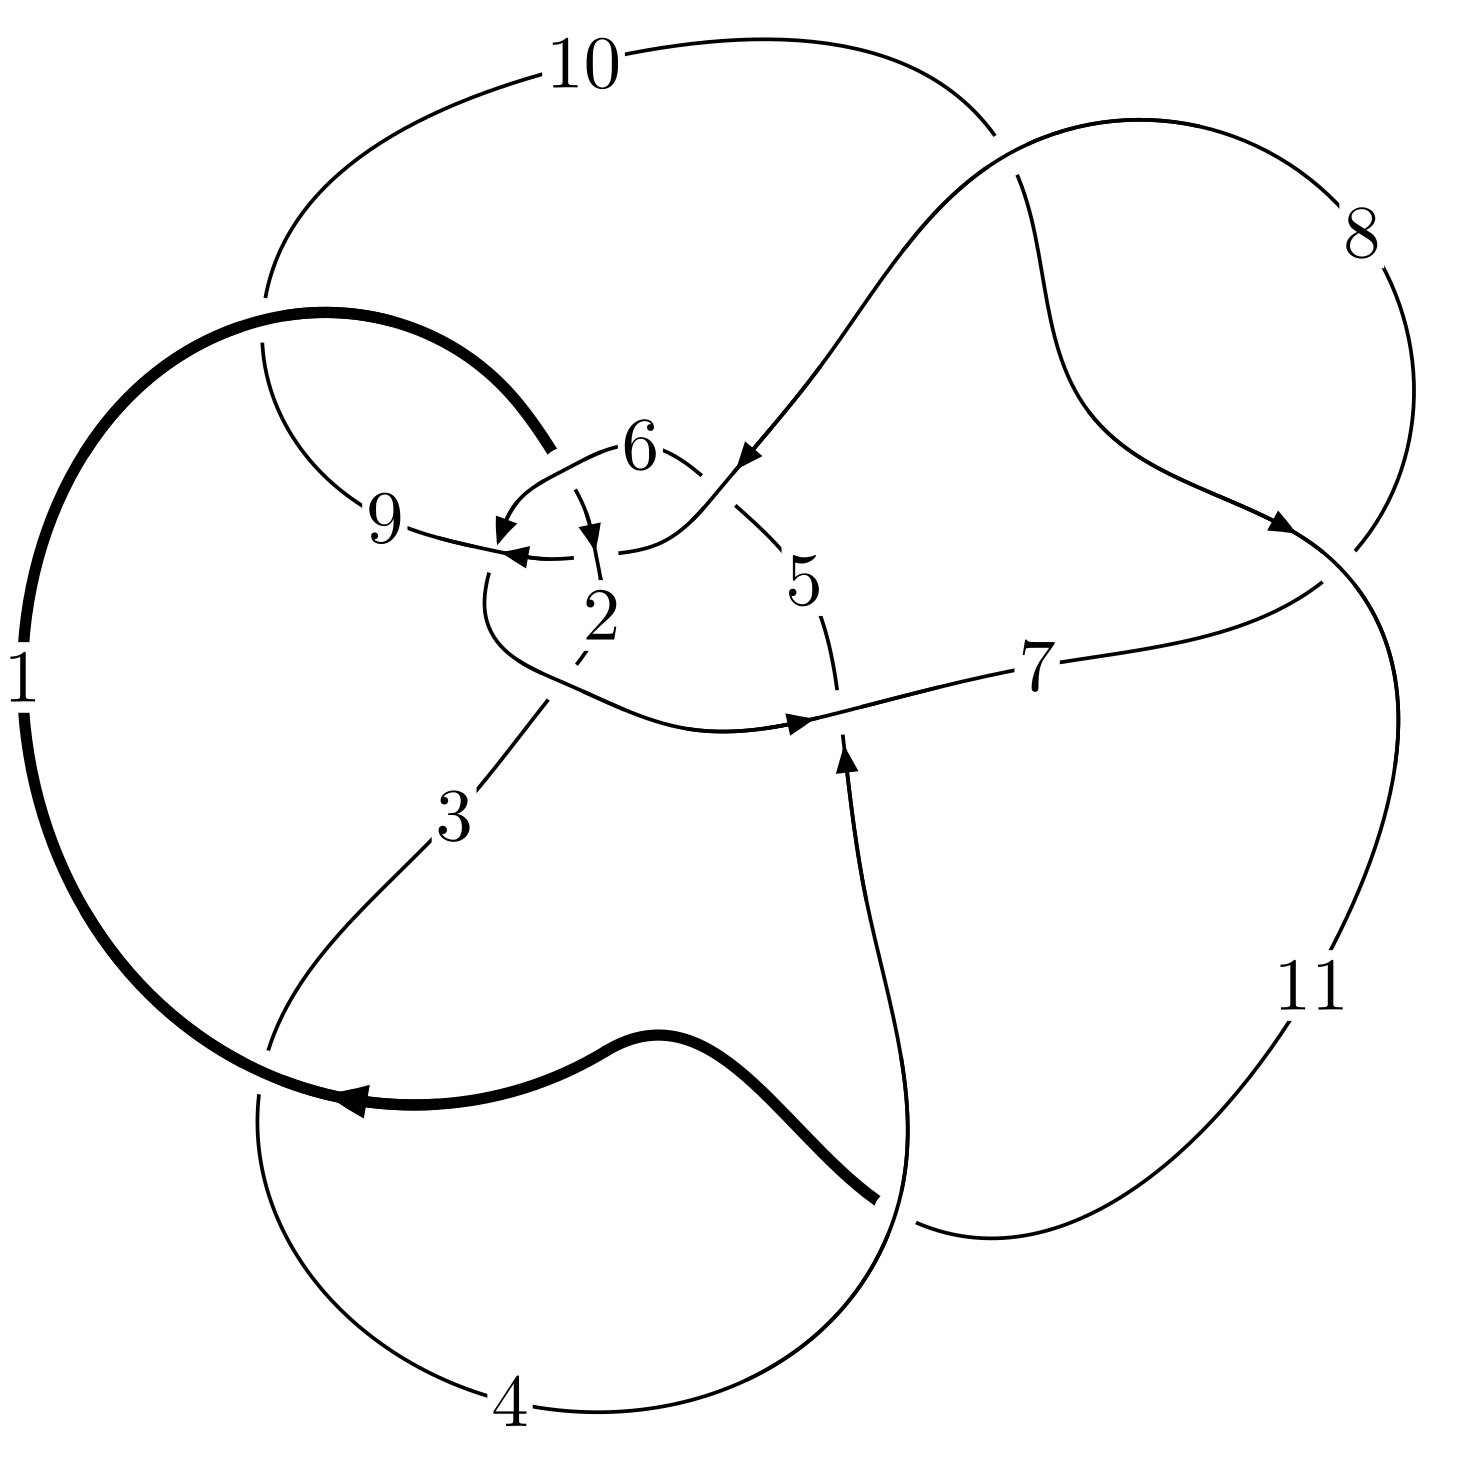
\includegraphics[width=112pt]{../../../GIT/diagram.site/Diagrams/png/779_11n_163.png}\\
\ \ \ A knot diagram\footnotemark}&
\allowdisplaybreaks
\textbf{Linearized knot diagam} \\
\cline{2-2}
 &
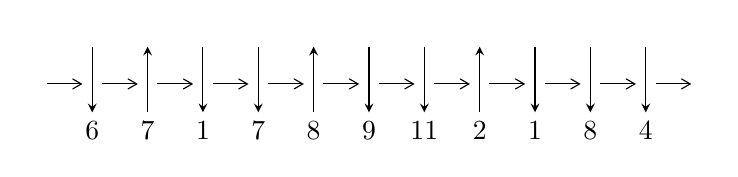
\begin{tikzpicture}[x=20pt, y=17pt]
	% nodes
	\node (C0) at (0, 0) {};
	\node (C1) at (1, 0) {};
	\node (C1U) at (1, +1) {};
	\node (C1D) at (1, -1) {6};

	\node (C2) at (2, 0) {};
	\node (C2U) at (2, +1) {};
	\node (C2D) at (2, -1) {7};

	\node (C3) at (3, 0) {};
	\node (C3U) at (3, +1) {};
	\node (C3D) at (3, -1) {1};

	\node (C4) at (4, 0) {};
	\node (C4U) at (4, +1) {};
	\node (C4D) at (4, -1) {7};

	\node (C5) at (5, 0) {};
	\node (C5U) at (5, +1) {};
	\node (C5D) at (5, -1) {8};

	\node (C6) at (6, 0) {};
	\node (C6U) at (6, +1) {};
	\node (C6D) at (6, -1) {9};

	\node (C7) at (7, 0) {};
	\node (C7U) at (7, +1) {};
	\node (C7D) at (7, -1) {11};

	\node (C8) at (8, 0) {};
	\node (C8U) at (8, +1) {};
	\node (C8D) at (8, -1) {2};

	\node (C9) at (9, 0) {};
	\node (C9U) at (9, +1) {};
	\node (C9D) at (9, -1) {1};

	\node (C10) at (10, 0) {};
	\node (C10U) at (10, +1) {};
	\node (C10D) at (10, -1) {8};

	\node (C11) at (11, 0) {};
	\node (C11U) at (11, +1) {};
	\node (C11D) at (11, -1) {4};
	\node (C12) at (12, 0) {};

	% arrows
	\draw[->,>={angle 60}]
	(C0) edge (C1) (C1) edge (C2) (C2) edge (C3) (C3) edge (C4) (C4) edge (C5) (C5) edge (C6) (C6) edge (C7) (C7) edge (C8) (C8) edge (C9) (C9) edge (C10) (C10) edge (C11) (C11) edge (C12) ;	\draw[->,>=stealth]
	(C1U) edge (C1D) (C2D) edge (C2U) (C3U) edge (C3D) (C4U) edge (C4D) (C5D) edge (C5U) (C6U) edge (C6D) (C7U) edge (C7D) (C8D) edge (C8U) (C9U) edge (C9D) (C10U) edge (C10D) (C11U) edge (C11D) ;
	\end{tikzpicture} \\
\hhline{~~} \\& 
\textbf{Solving Sequence} \\ \cline{2-2} 
 &
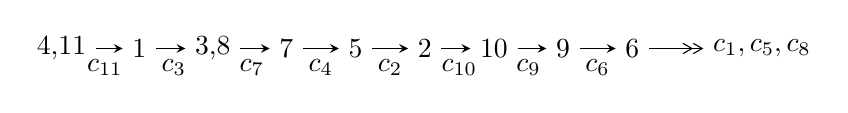
\begin{tikzpicture}[x=25pt, y=7pt]
	% node
	\node (A0) at (-1/8, 0) {4,11};
	\node (A1) at (1, 0) {1};
	\node (A2) at (33/16, 0) {3,8};
	\node (A3) at (25/8, 0) {7};
	\node (A4) at (33/8, 0) {5};
	\node (A5) at (41/8, 0) {2};
	\node (A6) at (49/8, 0) {10};
	\node (A7) at (57/8, 0) {9};
	\node (A8) at (65/8, 0) {6};
	\node (C1) at (1/2, -1) {$c_{11}$};
	\node (C2) at (3/2, -1) {$c_{3}$};
	\node (C3) at (21/8, -1) {$c_{7}$};
	\node (C4) at (29/8, -1) {$c_{4}$};
	\node (C5) at (37/8, -1) {$c_{2}$};
	\node (C6) at (45/8, -1) {$c_{10}$};
	\node (C7) at (53/8, -1) {$c_{9}$};
	\node (C8) at (61/8, -1) {$c_{6}$};
	\node (A9) at (10, 0) {$c_{1},c_{5},c_{8}$};

	% edge
	\draw[->,>=stealth]	
	(A0) edge (A1) (A1) edge (A2) (A2) edge (A3) (A3) edge (A4) (A4) edge (A5) (A5) edge (A6) (A6) edge (A7) (A7) edge (A8) ;
	\draw[->>,>={angle 60}]	
	(A8) edge (A9);
\end{tikzpicture} \\ 

\end{tabular} \\

\footnotetext{
The image of knot diagram is generated by the software ``\textbf{Draw programme}" developed by Andrew Bartholomew(\url{http://www.layer8.co.uk/maths/draw/index.htm\#Running-draw}), where we modified some parts for our purpose(\url{https://github.com/CATsTAILs/LinksPainter}).
}\phantom \\ \newline 
\centering \textbf{Ideals for irreducible components\footnotemark of $X_{\text{par}}$} 
 
\begin{align*}
I^u_{1}&=\langle 
b- u,\;-45168 u^{15}+5735 u^{14}+\cdots+12553 a-4016,\\
\phantom{I^u_{1}}&\phantom{= \langle  }u^{16}+4 u^{14}+13 u^{12}+25 u^{10}+37 u^8+u^7+39 u^6+5 u^5+24 u^4+7 u^3+8 u^2+2 u+1\rangle \\
I^u_{2}&=\langle 
9.55720\times10^{54} u^{41}+1.20936\times10^{55} u^{40}+\cdots+1.06854\times10^{57} b+1.17356\times10^{57},\\
\phantom{I^u_{2}}&\phantom{= \langle  }1.73442\times10^{56} u^{41}+5.21769\times10^{56} u^{40}+\cdots+1.06854\times10^{57} a+1.20542\times10^{58},\;u^{42}+3 u^{41}+\cdots+36 u-1\rangle \\
I^u_{3}&=\langle 
b+u,\;2 u^6-4 u^5+7 u^4-6 u^3+4 u^2+a- u-1,\;u^7-2 u^6+4 u^5-4 u^4+4 u^3-2 u^2+u-1\rangle \\
I^u_{4}&=\langle 
- u^5+2 u^4-4 u^3+5 u^2+b-4 u+2,\;- u^4+2 u^3-4 u^2+a+5 u-3,\;u^6-2 u^5+4 u^4-5 u^3+4 u^2-2 u+1\rangle \\
\\
\end{align*}
\raggedright * 4 irreducible components of $\dim_{\mathbb{C}}=0$, with total 71 representations.\\
\footnotetext{All coefficients of polynomials are rational numbers. But the coefficients are sometimes approximated in decimal forms when there is not enough margin.}
\newpage
\renewcommand{\arraystretch}{1}
\centering \section*{I. $I^u_{1}= \langle b- u,\;-45168 u^{15}+5735 u^{14}+\cdots+12553 a-4016,\;u^{16}+4 u^{14}+\cdots+2 u+1 \rangle$}
\flushleft \textbf{(i) Arc colorings}\\
\begin{tabular}{m{7pt} m{180pt} m{7pt} m{180pt} }
\flushright $a_{4}=$&$\begin{pmatrix}0\\u\end{pmatrix}$ \\
\flushright $a_{11}=$&$\begin{pmatrix}1\\0\end{pmatrix}$ \\
\flushright $a_{1}=$&$\begin{pmatrix}1\\u^2\end{pmatrix}$ \\
\flushright $a_{3}=$&$\begin{pmatrix}u\\u^3+u\end{pmatrix}$ \\
\flushright $a_{8}=$&$\begin{pmatrix}3.59818 u^{15}-0.456863 u^{14}+\cdots+6.71059 u+0.319924\\u\end{pmatrix}$ \\
\flushright $a_{7}=$&$\begin{pmatrix}3.59818 u^{15}-0.456863 u^{14}+\cdots+7.71059 u+0.319924\\u\end{pmatrix}$ \\
\flushright $a_{5}=$&$\begin{pmatrix}-2.45439 u^{15}-4.20816 u^{14}+\cdots-29.2987 u-12.3139\\1.39951 u^{15}-0.238270 u^{14}+\cdots+3.68446 u-0.456863\end{pmatrix}$ \\
\flushright $a_{2}=$&$\begin{pmatrix}-2.66016 u^{15}-2.57118 u^{14}+\cdots-20.1125 u-7.64885\\0.808412 u^{15}-0.199793 u^{14}+\cdots+2.76149 u-0.218593\end{pmatrix}$ \\
\flushright $a_{10}=$&$\begin{pmatrix}0.456863 u^{15}+1.39951 u^{14}+\cdots+6.87644 u+4.59818\\- u^2\end{pmatrix}$ \\
\flushright $a_{9}=$&$\begin{pmatrix}0.695133 u^{15}+1.99060 u^{14}+\cdots+10.1323 u+5.99769\\-0.0384769 u^{15}-0.336175 u^{14}+\cdots-1.42046 u-0.591094\end{pmatrix}$ \\
\flushright $a_{6}=$&$\begin{pmatrix}1.01418 u^{15}-1.83677 u^{14}+\cdots-6.42476 u-4.88361\\0.591094 u^{15}-0.0384769 u^{14}+\cdots+1.92297 u-0.238270\end{pmatrix}$\\ \flushright $a_{6}=$&$\begin{pmatrix}1.01418 u^{15}-1.83677 u^{14}+\cdots-6.42476 u-4.88361\\0.591094 u^{15}-0.0384769 u^{14}+\cdots+1.92297 u-0.238270\end{pmatrix}$\\&\end{tabular}
\flushleft \textbf{(ii) Obstruction class $= -1$}\\~\\
\flushleft \textbf{(iii) Cusp Shapes $= -\frac{31115}{12553} u^{15}+\frac{20322}{12553} u^{14}+\cdots-\frac{177549}{12553} u-\frac{9899}{12553}$}\\~\\
\newpage\renewcommand{\arraystretch}{1}
\flushleft \textbf{(iv) u-Polynomials at the component}\newline \\
\begin{tabular}{m{50pt}|m{274pt}}
Crossings & \hspace{64pt}u-Polynomials at each crossing \\
\hline $$\begin{aligned}c_{1},c_{6}\end{aligned}$$&$\begin{aligned}
&u^{16}- u^{15}+\cdots- u+1
\end{aligned}$\\
\hline $$\begin{aligned}c_{2},c_{5}\end{aligned}$$&$\begin{aligned}
&u^{16}- u^{15}+\cdots+15 u^2+1
\end{aligned}$\\
\hline $$\begin{aligned}c_{3},c_{7},c_{10}\\c_{11}\end{aligned}$$&$\begin{aligned}
&u^{16}+4 u^{14}+\cdots+2 u+1
\end{aligned}$\\
\hline $$\begin{aligned}c_{4}\end{aligned}$$&$\begin{aligned}
&u^{16}-13 u^{15}+\cdots-352 u+64
\end{aligned}$\\
\hline $$\begin{aligned}c_{8}\end{aligned}$$&$\begin{aligned}
&u^{16}-13 u^{15}+\cdots-36 u+8
\end{aligned}$\\
\hline $$\begin{aligned}c_{9}\end{aligned}$$&$\begin{aligned}
&u^{16}-16 u^{15}+\cdots-544 u+64
\end{aligned}$\\
\hline
\end{tabular}\\~\\
\newpage\renewcommand{\arraystretch}{1}
\flushleft \textbf{(v) Riley Polynomials at the component}\newline \\
\begin{tabular}{m{50pt}|m{274pt}}
Crossings & \hspace{64pt}Riley Polynomials at each crossing \\
\hline $$\begin{aligned}c_{1},c_{6}\end{aligned}$$&$\begin{aligned}
&y^{16}-3 y^{15}+\cdots-5 y+1
\end{aligned}$\\
\hline $$\begin{aligned}c_{2},c_{5}\end{aligned}$$&$\begin{aligned}
&y^{16}+9 y^{15}+\cdots+30 y+1
\end{aligned}$\\
\hline $$\begin{aligned}c_{3},c_{7},c_{10}\\c_{11}\end{aligned}$$&$\begin{aligned}
&y^{16}+8 y^{15}+\cdots+12 y+1
\end{aligned}$\\
\hline $$\begin{aligned}c_{4}\end{aligned}$$&$\begin{aligned}
&y^{16}+5 y^{15}+\cdots+40448 y+4096
\end{aligned}$\\
\hline $$\begin{aligned}c_{8}\end{aligned}$$&$\begin{aligned}
&y^{16}- y^{15}+\cdots+496 y+64
\end{aligned}$\\
\hline $$\begin{aligned}c_{9}\end{aligned}$$&$\begin{aligned}
&y^{16}-4 y^{15}+\cdots+23552 y+4096
\end{aligned}$\\
\hline
\end{tabular}\\~\\
\newpage\flushleft \textbf{(vi) Complex Volumes and Cusp Shapes}
$$\begin{array}{c|c|c}  
\text{Solutions to }I^u_{1}& \I (\text{vol} + \sqrt{-1}CS) & \text{Cusp shape}\\
 \hline 
\begin{aligned}
u &= \phantom{-}0.362872 + 0.921754 I \\
a &= \phantom{-}0.762991 - 0.560929 I \\
b &= \phantom{-}0.362872 + 0.921754 I\end{aligned}
 & \phantom{-}3.94475 + 1.12356 I & \phantom{-}1.32088 + 0.73756 I \\ \hline\begin{aligned}
u &= \phantom{-}0.362872 - 0.921754 I \\
a &= \phantom{-}0.762991 + 0.560929 I \\
b &= \phantom{-}0.362872 - 0.921754 I\end{aligned}
 & \phantom{-}3.94475 - 1.12356 I & \phantom{-}1.32088 - 0.73756 I \\ \hline\begin{aligned}
u &= -0.067924 + 1.048980 I \\
a &= \phantom{-}0.59848 - 1.57127 I \\
b &= -0.067924 + 1.048980 I\end{aligned}
 & \phantom{-}3.11555 + 2.14731 I & -0.93627 - 3.92704 I \\ \hline\begin{aligned}
u &= -0.067924 - 1.048980 I \\
a &= \phantom{-}0.59848 + 1.57127 I \\
b &= -0.067924 - 1.048980 I\end{aligned}
 & \phantom{-}3.11555 - 2.14731 I & -0.93627 + 3.92704 I \\ \hline\begin{aligned}
u &= \phantom{-}0.867369 + 0.851352 I \\
a &= \phantom{-}0.39653 - 1.47637 I \\
b &= \phantom{-}0.867369 + 0.851352 I\end{aligned}
 & -4.45687 + 2.76976 I & -6.60351 - 1.02062 I \\ \hline\begin{aligned}
u &= \phantom{-}0.867369 - 0.851352 I \\
a &= \phantom{-}0.39653 + 1.47637 I \\
b &= \phantom{-}0.867369 - 0.851352 I\end{aligned}
 & -4.45687 - 2.76976 I & -6.60351 + 1.02062 I \\ \hline\begin{aligned}
u &= -0.924080 + 0.993395 I \\
a &= -0.062325 - 1.181310 I \\
b &= -0.924080 + 0.993395 I\end{aligned}
 & -2.56347 + 5.89381 I & -14.0887 - 6.8568 I \\ \hline\begin{aligned}
u &= -0.924080 - 0.993395 I \\
a &= -0.062325 + 1.181310 I \\
b &= -0.924080 - 0.993395 I\end{aligned}
 & -2.56347 - 5.89381 I & -14.0887 + 6.8568 I \\ \hline\begin{aligned}
u &= -0.037947 + 0.609427 I \\
a &= -4.09907 - 0.73703 I \\
b &= -0.037947 + 0.609427 I\end{aligned}
 & \phantom{-}0.98282 - 4.26271 I & -0.536037 - 0.693456 I \\ \hline\begin{aligned}
u &= -0.037947 - 0.609427 I \\
a &= -4.09907 + 0.73703 I \\
b &= -0.037947 - 0.609427 I\end{aligned}
 & \phantom{-}0.98282 + 4.26271 I & -0.536037 + 0.693456 I\\
 \hline 
 \end{array}$$\newpage$$\begin{array}{c|c|c}  
\text{Solutions to }I^u_{1}& \I (\text{vol} + \sqrt{-1}CS) & \text{Cusp shape}\\
 \hline 
\begin{aligned}
u &= -0.74781 + 1.20294 I \\
a &= -0.21869 - 1.80308 I \\
b &= -0.74781 + 1.20294 I\end{aligned}
 & -0.89621 + 7.24124 I & -3.27217 - 13.36826 I \\ \hline\begin{aligned}
u &= -0.74781 - 1.20294 I \\
a &= -0.21869 + 1.80308 I \\
b &= -0.74781 - 1.20294 I\end{aligned}
 & -0.89621 - 7.24124 I & -3.27217 + 13.36826 I \\ \hline\begin{aligned}
u &= \phantom{-}0.82584 + 1.20295 I \\
a &= \phantom{-}0.47696 - 1.60926 I \\
b &= \phantom{-}0.82584 + 1.20295 I\end{aligned}
 & -2.2047 - 16.1487 I & -3.69661 + 9.09082 I \\ \hline\begin{aligned}
u &= \phantom{-}0.82584 - 1.20295 I \\
a &= \phantom{-}0.47696 + 1.60926 I \\
b &= \phantom{-}0.82584 - 1.20295 I\end{aligned}
 & -2.2047 + 16.1487 I & -3.69661 - 9.09082 I \\ \hline\begin{aligned}
u &= -0.278326 + 0.368111 I \\
a &= \phantom{-}1.14513 - 0.86473 I \\
b &= -0.278326 + 0.368111 I\end{aligned}
 & -0.389238 + 1.281380 I & -3.68762 - 5.53338 I \\ \hline\begin{aligned}
u &= -0.278326 - 0.368111 I \\
a &= \phantom{-}1.14513 + 0.86473 I \\
b &= -0.278326 - 0.368111 I\end{aligned}
 & -0.389238 - 1.281380 I & -3.68762 + 5.53338 I\\
 \hline 
 \end{array}$$\newpage\newpage\renewcommand{\arraystretch}{1}
\centering \section*{II. $I^u_{2}= \langle 9.56\times10^{54} u^{41}+1.21\times10^{55} u^{40}+\cdots+1.07\times10^{57} b+1.17\times10^{57},\;1.73\times10^{56} u^{41}+5.22\times10^{56} u^{40}+\cdots+1.07\times10^{57} a+1.21\times10^{58},\;u^{42}+3 u^{41}+\cdots+36 u-1 \rangle$}
\flushleft \textbf{(i) Arc colorings}\\
\begin{tabular}{m{7pt} m{180pt} m{7pt} m{180pt} }
\flushright $a_{4}=$&$\begin{pmatrix}0\\u\end{pmatrix}$ \\
\flushright $a_{11}=$&$\begin{pmatrix}1\\0\end{pmatrix}$ \\
\flushright $a_{1}=$&$\begin{pmatrix}1\\u^2\end{pmatrix}$ \\
\flushright $a_{3}=$&$\begin{pmatrix}u\\u^3+u\end{pmatrix}$ \\
\flushright $a_{8}=$&$\begin{pmatrix}-0.162317 u^{41}-0.488303 u^{40}+\cdots+6.42121 u-11.2810\\-0.00894419 u^{41}-0.0113179 u^{40}+\cdots-3.72593 u-1.09829\end{pmatrix}$ \\
\flushright $a_{7}=$&$\begin{pmatrix}-0.171261 u^{41}-0.499621 u^{40}+\cdots+2.69528 u-12.3793\\-0.00894419 u^{41}-0.0113179 u^{40}+\cdots-3.72593 u-1.09829\end{pmatrix}$ \\
\flushright $a_{5}=$&$\begin{pmatrix}0.0765764 u^{41}+0.218473 u^{40}+\cdots-9.92664 u-3.95597\\0.0117602 u^{41}+0.0207404 u^{40}+\cdots-5.71991 u-0.217988\end{pmatrix}$ \\
\flushright $a_{2}=$&$\begin{pmatrix}0.0458921 u^{41}+0.116885 u^{40}+\cdots-1.72493 u-3.74924\\-0.00981888 u^{41}-0.0511014 u^{40}+\cdots-3.81460 u-0.236598\end{pmatrix}$ \\
\flushright $a_{10}=$&$\begin{pmatrix}-0.222058 u^{41}-0.640758 u^{40}+\cdots-2.30612 u-12.3439\\0.00407009 u^{41}-0.00144471 u^{40}+\cdots-7.80288 u-1.22358\end{pmatrix}$ \\
\flushright $a_{9}=$&$\begin{pmatrix}-0.234716 u^{41}-0.693689 u^{40}+\cdots-8.97199 u-13.5929\\-0.0134003 u^{41}-0.0709336 u^{40}+\cdots-7.27710 u-1.23853\end{pmatrix}$ \\
\flushright $a_{6}=$&$\begin{pmatrix}0.245729 u^{41}+0.839363 u^{40}+\cdots+9.37284 u+4.46731\\0.0686483 u^{41}+0.146810 u^{40}+\cdots-6.32759 u+0.755792\end{pmatrix}$\\ \flushright $a_{6}=$&$\begin{pmatrix}0.245729 u^{41}+0.839363 u^{40}+\cdots+9.37284 u+4.46731\\0.0686483 u^{41}+0.146810 u^{40}+\cdots-6.32759 u+0.755792\end{pmatrix}$\\&\end{tabular}
\flushleft \textbf{(ii) Obstruction class $= -1$}\\~\\
\flushleft \textbf{(iii) Cusp Shapes $= 0.445546 u^{41}+1.05637 u^{40}+\cdots-7.66940 u+9.51539$}\\~\\
\newpage\renewcommand{\arraystretch}{1}
\flushleft \textbf{(iv) u-Polynomials at the component}\newline \\
\begin{tabular}{m{50pt}|m{274pt}}
Crossings & \hspace{64pt}u-Polynomials at each crossing \\
\hline $$\begin{aligned}c_{1},c_{6}\end{aligned}$$&$\begin{aligned}
&u^{42}- u^{41}+\cdots-7 u-1
\end{aligned}$\\
\hline $$\begin{aligned}c_{2},c_{5}\end{aligned}$$&$\begin{aligned}
&u^{42}+7 u^{40}+\cdots+1895 u+457
\end{aligned}$\\
\hline $$\begin{aligned}c_{3},c_{7},c_{10}\\c_{11}\end{aligned}$$&$\begin{aligned}
&u^{42}+3 u^{41}+\cdots+36 u-1
\end{aligned}$\\
\hline $$\begin{aligned}c_{4}\end{aligned}$$&$\begin{aligned}
&(u^{21}+8 u^{20}+\cdots+43 u+7)^{2}
\end{aligned}$\\
\hline $$\begin{aligned}c_{8}\end{aligned}$$&$\begin{aligned}
&(u^{21}+6 u^{20}+\cdots+5 u+1)^{2}
\end{aligned}$\\
\hline $$\begin{aligned}c_{9}\end{aligned}$$&$\begin{aligned}
&(u^{21}+6 u^{20}+\cdots+9 u+1)^{2}
\end{aligned}$\\
\hline
\end{tabular}\\~\\
\newpage\renewcommand{\arraystretch}{1}
\flushleft \textbf{(v) Riley Polynomials at the component}\newline \\
\begin{tabular}{m{50pt}|m{274pt}}
Crossings & \hspace{64pt}Riley Polynomials at each crossing \\
\hline $$\begin{aligned}c_{1},c_{6}\end{aligned}$$&$\begin{aligned}
&y^{42}- y^{41}+\cdots-45 y+1
\end{aligned}$\\
\hline $$\begin{aligned}c_{2},c_{5}\end{aligned}$$&$\begin{aligned}
&y^{42}+14 y^{41}+\cdots+2544657 y+208849
\end{aligned}$\\
\hline $$\begin{aligned}c_{3},c_{7},c_{10}\\c_{11}\end{aligned}$$&$\begin{aligned}
&y^{42}+11 y^{41}+\cdots-1288 y+1
\end{aligned}$\\
\hline $$\begin{aligned}c_{4}\end{aligned}$$&$\begin{aligned}
&(y^{21}-10 y^{20}+\cdots+1149 y-49)^{2}
\end{aligned}$\\
\hline $$\begin{aligned}c_{8}\end{aligned}$$&$\begin{aligned}
&(y^{21}+2 y^{20}+\cdots-11 y-1)^{2}
\end{aligned}$\\
\hline $$\begin{aligned}c_{9}\end{aligned}$$&$\begin{aligned}
&(y^{21}-8 y^{20}+\cdots+33 y-1)^{2}
\end{aligned}$\\
\hline
\end{tabular}\\~\\
\newpage\flushleft \textbf{(vi) Complex Volumes and Cusp Shapes}
$$\begin{array}{c|c|c}  
\text{Solutions to }I^u_{2}& \I (\text{vol} + \sqrt{-1}CS) & \text{Cusp shape}\\
 \hline 
\begin{aligned}
u &= -0.885119 + 0.440669 I \\
a &= \phantom{-}0.437217 + 0.545665 I \\
b &= -0.998691 - 0.783756 I\end{aligned}
 & -3.16717 - 1.07030 I & -12.89268 + 5.67416 I \\ \hline\begin{aligned}
u &= -0.885119 - 0.440669 I \\
a &= \phantom{-}0.437217 - 0.545665 I \\
b &= -0.998691 + 0.783756 I\end{aligned}
 & -3.16717 + 1.07030 I & -12.89268 - 5.67416 I \\ \hline\begin{aligned}
u &= -0.221318 + 0.954664 I \\
a &= \phantom{-}1.023340 + 0.577719 I \\
b &= \phantom{-}0.715301 - 0.650320 I\end{aligned}
 & \phantom{-}2.51518 + 5.37801 I & \phantom{-}0.71786 - 8.23406 I \\ \hline\begin{aligned}
u &= -0.221318 - 0.954664 I \\
a &= \phantom{-}1.023340 - 0.577719 I \\
b &= \phantom{-}0.715301 + 0.650320 I\end{aligned}
 & \phantom{-}2.51518 - 5.37801 I & \phantom{-}0.71786 + 8.23406 I \\ \hline\begin{aligned}
u &= \phantom{-}0.715301 + 0.650320 I \\
a &= -1.186310 - 0.108494 I \\
b &= -0.221318 - 0.954664 I\end{aligned}
 & \phantom{-}2.51518 - 5.37801 I & \phantom{-}0.71786 + 8.23406 I \\ \hline\begin{aligned}
u &= \phantom{-}0.715301 - 0.650320 I \\
a &= -1.186310 + 0.108494 I \\
b &= -0.221318 + 0.954664 I\end{aligned}
 & \phantom{-}2.51518 + 5.37801 I & \phantom{-}0.71786 - 8.23406 I \\ \hline\begin{aligned}
u &= \phantom{-}0.660616 + 0.665590 I \\
a &= \phantom{-}0.142774 + 0.166906 I \\
b &= -1.181090 + 0.555383 I\end{aligned}
 & -3.87464 - 0.10689 I & -16.3307 + 2.6685 I \\ \hline\begin{aligned}
u &= \phantom{-}0.660616 - 0.665590 I \\
a &= \phantom{-}0.142774 - 0.166906 I \\
b &= -1.181090 - 0.555383 I\end{aligned}
 & -3.87464 + 0.10689 I & -16.3307 - 2.6685 I \\ \hline\begin{aligned}
u &= \phantom{-}0.746526 + 0.760439 I \\
a &= \phantom{-}0.567031 - 0.156980 I \\
b &= -0.884140 + 0.948082 I\end{aligned}
 & -2.33356 + 1.75773 I & -7.03716 - 6.33959 I \\ \hline\begin{aligned}
u &= \phantom{-}0.746526 - 0.760439 I \\
a &= \phantom{-}0.567031 + 0.156980 I \\
b &= -0.884140 - 0.948082 I\end{aligned}
 & -2.33356 - 1.75773 I & -7.03716 + 6.33959 I\\
 \hline 
 \end{array}$$\newpage$$\begin{array}{c|c|c}  
\text{Solutions to }I^u_{2}& \I (\text{vol} + \sqrt{-1}CS) & \text{Cusp shape}\\
 \hline 
\begin{aligned}
u &= -0.549689 + 0.965680 I \\
a &= \phantom{-}1.164290 + 0.499543 I \\
b &= -0.011102 - 0.408161 I\end{aligned}
 & \phantom{-}0.21083 + 2.02252 I & -3.27794 - 3.16369 I \\ \hline\begin{aligned}
u &= -0.549689 - 0.965680 I \\
a &= \phantom{-}1.164290 - 0.499543 I \\
b &= -0.011102 + 0.408161 I\end{aligned}
 & \phantom{-}0.21083 - 2.02252 I & -3.27794 + 3.16369 I \\ \hline\begin{aligned}
u &= \phantom{-}0.587817 + 1.024500 I \\
a &= -0.44869 + 1.75524 I \\
b &= -0.903022 - 0.809434 I\end{aligned}
 & -2.75188 - 4.82047 I & -10.54242 + 4.40996 I \\ \hline\begin{aligned}
u &= \phantom{-}0.587817 - 1.024500 I \\
a &= -0.44869 - 1.75524 I \\
b &= -0.903022 + 0.809434 I\end{aligned}
 & -2.75188 + 4.82047 I & -10.54242 - 4.40996 I \\ \hline\begin{aligned}
u &= \phantom{-}0.112117 + 0.790036 I \\
a &= \phantom{-}0.80867 - 3.05059 I \\
b &= -0.175620 + 1.395210 I\end{aligned}
 & \phantom{-}5.06212 + 3.17952 I & \phantom{-}3.66314 + 2.07098 I \\ \hline\begin{aligned}
u &= \phantom{-}0.112117 - 0.790036 I \\
a &= \phantom{-}0.80867 + 3.05059 I \\
b &= -0.175620 - 1.395210 I\end{aligned}
 & \phantom{-}5.06212 - 3.17952 I & \phantom{-}3.66314 - 2.07098 I \\ \hline\begin{aligned}
u &= \phantom{-}0.716213 + 0.968774 I \\
a &= -0.72128 + 1.60893 I \\
b &= -0.84147 - 1.24514 I\end{aligned}
 & -1.69311 - 7.34221 I & -7.2251 + 12.7560 I \\ \hline\begin{aligned}
u &= \phantom{-}0.716213 - 0.968774 I \\
a &= -0.72128 - 1.60893 I \\
b &= -0.84147 + 1.24514 I\end{aligned}
 & -1.69311 + 7.34221 I & -7.2251 - 12.7560 I \\ \hline\begin{aligned}
u &= -1.20681\phantom{ +0.000000I} \\
a &= \phantom{-}0.255916\phantom{ +0.000000I} \\
b &= \phantom{-}0.0276533\phantom{ +0.000000I}\end{aligned}
 & -2.39902\phantom{ +0.000000I} & \phantom{-}9.38220\phantom{ +0.000000I} \\ \hline\begin{aligned}
u &= -0.903022 + 0.809434 I \\
a &= \phantom{-}0.95127 + 1.48619 I \\
b &= \phantom{-}0.587817 - 1.024500 I\end{aligned}
 & -2.75188 + 4.82047 I & -10.54242 - 4.40996 I\\
 \hline 
 \end{array}$$\newpage$$\begin{array}{c|c|c}  
\text{Solutions to }I^u_{2}& \I (\text{vol} + \sqrt{-1}CS) & \text{Cusp shape}\\
 \hline 
\begin{aligned}
u &= -0.903022 - 0.809434 I \\
a &= \phantom{-}0.95127 - 1.48619 I \\
b &= \phantom{-}0.587817 + 1.024500 I\end{aligned}
 & -2.75188 - 4.82047 I & -10.54242 + 4.40996 I \\ \hline\begin{aligned}
u &= \phantom{-}0.280918 + 0.724094 I \\
a &= -0.42253 + 2.14926 I \\
b &= -0.06930 - 1.59935 I\end{aligned}
 & \phantom{-}4.77684 - 4.89958 I & -1.86079 + 9.83067 I \\ \hline\begin{aligned}
u &= \phantom{-}0.280918 - 0.724094 I \\
a &= -0.42253 - 2.14926 I \\
b &= -0.06930 + 1.59935 I\end{aligned}
 & \phantom{-}4.77684 + 4.89958 I & -1.86079 - 9.83067 I \\ \hline\begin{aligned}
u &= \phantom{-}0.819992 + 0.955539 I \\
a &= -0.487721 + 0.138368 I \\
b &= \phantom{-}1.170640 - 0.603687 I\end{aligned}
 & -4.12482 - 9.03603 I & -5.90532 + 6.27658 I \\ \hline\begin{aligned}
u &= \phantom{-}0.819992 - 0.955539 I \\
a &= -0.487721 - 0.138368 I \\
b &= \phantom{-}1.170640 + 0.603687 I\end{aligned}
 & -4.12482 + 9.03603 I & -5.90532 - 6.27658 I \\ \hline\begin{aligned}
u &= -0.998691 + 0.783756 I \\
a &= \phantom{-}0.529988 + 0.125234 I \\
b &= -0.885119 - 0.440669 I\end{aligned}
 & -3.16717 + 1.07030 I & -12.89268 - 5.67416 I \\ \hline\begin{aligned}
u &= -0.998691 - 0.783756 I \\
a &= \phantom{-}0.529988 - 0.125234 I \\
b &= -0.885119 + 0.440669 I\end{aligned}
 & -3.16717 - 1.07030 I & -12.89268 + 5.67416 I \\ \hline\begin{aligned}
u &= -0.884140 + 0.948082 I \\
a &= -0.108358 - 0.471345 I \\
b &= \phantom{-}0.746526 + 0.760439 I\end{aligned}
 & -2.33356 + 1.75773 I & -7.03716 - 6.33959 I \\ \hline\begin{aligned}
u &= -0.884140 - 0.948082 I \\
a &= -0.108358 + 0.471345 I \\
b &= \phantom{-}0.746526 - 0.760439 I\end{aligned}
 & -2.33356 - 1.75773 I & -7.03716 + 6.33959 I \\ \hline\begin{aligned}
u &= -1.181090 + 0.555383 I \\
a &= \phantom{-}0.078562 - 0.136872 I \\
b &= \phantom{-}0.660616 + 0.665590 I\end{aligned}
 & -3.87464 - 0.10689 I & -16.3307 + 2.6685 I\\
 \hline 
 \end{array}$$\newpage$$\begin{array}{c|c|c}  
\text{Solutions to }I^u_{2}& \I (\text{vol} + \sqrt{-1}CS) & \text{Cusp shape}\\
 \hline 
\begin{aligned}
u &= -1.181090 - 0.555383 I \\
a &= \phantom{-}0.078562 + 0.136872 I \\
b &= \phantom{-}0.660616 - 0.665590 I\end{aligned}
 & -3.87464 + 0.10689 I & -16.3307 - 2.6685 I \\ \hline\begin{aligned}
u &= \phantom{-}1.170640 + 0.603687 I \\
a &= -0.236393 + 0.423087 I \\
b &= \phantom{-}0.819992 - 0.955539 I\end{aligned}
 & -4.12482 + 9.03603 I & -5.90532 - 6.27658 I \\ \hline\begin{aligned}
u &= \phantom{-}1.170640 - 0.603687 I \\
a &= -0.236393 - 0.423087 I \\
b &= \phantom{-}0.819992 + 0.955539 I\end{aligned}
 & -4.12482 - 9.03603 I & -5.90532 + 6.27658 I \\ \hline\begin{aligned}
u &= -0.175620 + 1.395210 I \\
a &= -0.01264 - 1.79079 I \\
b &= \phantom{-}0.112117 + 0.790036 I\end{aligned}
 & \phantom{-}5.06212 + 3.17952 I & \phantom{-}3.66314 + 2.07098 I \\ \hline\begin{aligned}
u &= -0.175620 - 1.395210 I \\
a &= -0.01264 + 1.79079 I \\
b &= \phantom{-}0.112117 - 0.790036 I\end{aligned}
 & \phantom{-}5.06212 - 3.17952 I & \phantom{-}3.66314 - 2.07098 I \\ \hline\begin{aligned}
u &= -0.84147 + 1.24514 I \\
a &= \phantom{-}0.523153 + 1.313150 I \\
b &= \phantom{-}0.716213 - 0.968774 I\end{aligned}
 & -1.69311 + 7.34221 I & \phantom{-0.000000 } 0. - 12.75605 I \\ \hline\begin{aligned}
u &= -0.84147 - 1.24514 I \\
a &= \phantom{-}0.523153 - 1.313150 I \\
b &= \phantom{-}0.716213 + 0.968774 I\end{aligned}
 & -1.69311 - 7.34221 I & \phantom{-0.000000 -}0. + 12.75605 I \\ \hline\begin{aligned}
u &= -0.011102 + 0.408161 I \\
a &= -2.00560 + 2.80444 I \\
b &= -0.549689 - 0.965680 I\end{aligned}
 & \phantom{-}0.21083 - 2.02252 I & -3.27794 + 3.16369 I \\ \hline\begin{aligned}
u &= -0.011102 - 0.408161 I \\
a &= -2.00560 - 2.80444 I \\
b &= -0.549689 + 0.965680 I\end{aligned}
 & \phantom{-}0.21083 + 2.02252 I & -3.27794 - 3.16369 I \\ \hline\begin{aligned}
u &= -0.06930 + 1.59935 I \\
a &= -0.140568 + 1.053370 I \\
b &= \phantom{-}0.280918 - 0.724094 I\end{aligned}
 & \phantom{-}4.77684 + 4.89958 I & \phantom{-0.000000 } 0\\
 \hline 
 \end{array}$$\newpage$$\begin{array}{c|c|c}  
\text{Solutions to }I^u_{2}& \I (\text{vol} + \sqrt{-1}CS) & \text{Cusp shape}\\
 \hline 
\begin{aligned}
u &= -0.06930 - 1.59935 I \\
a &= -0.140568 - 1.053370 I \\
b &= \phantom{-}0.280918 + 0.724094 I\end{aligned}
 & \phantom{-}4.77684 - 4.89958 I & \phantom{-0.000000 } 0 \\ \hline\begin{aligned}
u &= \phantom{-}0.0276533\phantom{ +0.000000I} \\
a &= -11.1684\phantom{ +0.000000I} \\
b &= -1.20681\phantom{ +0.000000I}\end{aligned}
 & -2.39902\phantom{ +0.000000I} & \phantom{-}9.38220\phantom{ +0.000000I}\\
 \hline 
 \end{array}$$\newpage\newpage\renewcommand{\arraystretch}{1}
\centering \section*{III. $I^u_{3}= \langle b+u,\;2 u^6-4 u^5+7 u^4-6 u^3+4 u^2+a- u-1,\;u^7-2 u^6+4 u^5-4 u^4+4 u^3-2 u^2+u-1 \rangle$}
\flushleft \textbf{(i) Arc colorings}\\
\begin{tabular}{m{7pt} m{180pt} m{7pt} m{180pt} }
\flushright $a_{4}=$&$\begin{pmatrix}0\\u\end{pmatrix}$ \\
\flushright $a_{11}=$&$\begin{pmatrix}1\\0\end{pmatrix}$ \\
\flushright $a_{1}=$&$\begin{pmatrix}1\\u^2\end{pmatrix}$ \\
\flushright $a_{3}=$&$\begin{pmatrix}u\\u^3+u\end{pmatrix}$ \\
\flushright $a_{8}=$&$\begin{pmatrix}-2 u^6+4 u^5-7 u^4+6 u^3-4 u^2+u+1\\- u\end{pmatrix}$ \\
\flushright $a_{7}=$&$\begin{pmatrix}-2 u^6+4 u^5-7 u^4+6 u^3-4 u^2+1\\- u\end{pmatrix}$ \\
\flushright $a_{5}=$&$\begin{pmatrix}-2 u^5+6 u^4-11 u^3+13 u^2-11 u+4\\u^6-2 u^5+4 u^4-4 u^3+3 u^2- u\end{pmatrix}$ \\
\flushright $a_{2}=$&$\begin{pmatrix}u^6-3 u^5+7 u^4-10 u^3+10 u^2-6 u+2\\u^6-2 u^5+3 u^4-2 u^3+2 u^2\end{pmatrix}$ \\
\flushright $a_{10}=$&$\begin{pmatrix}u^5-2 u^4+4 u^3-3 u^2+3 u-1\\- u^2\end{pmatrix}$ \\
\flushright $a_{9}=$&$\begin{pmatrix}u^5-3 u^4+5 u^3-5 u^2+4 u-2\\- u^6+u^5-2 u^4+u^3-2 u^2\end{pmatrix}$ \\
\flushright $a_{6}=$&$\begin{pmatrix}- u^5+2 u^4-4 u^3+5 u^2-5 u+2\\u^4- u^3+u^2\end{pmatrix}$\\ \flushright $a_{6}=$&$\begin{pmatrix}- u^5+2 u^4-4 u^3+5 u^2-5 u+2\\u^4- u^3+u^2\end{pmatrix}$\\&\end{tabular}
\flushleft \textbf{(ii) Obstruction class $= 1$}\\~\\
\flushleft \textbf{(iii) Cusp Shapes $= -4 u^6- u^5+2 u^4-16 u^3+11 u^2-14 u-1$}\\~\\
\newpage\renewcommand{\arraystretch}{1}
\flushleft \textbf{(iv) u-Polynomials at the component}\newline \\
\begin{tabular}{m{50pt}|m{274pt}}
Crossings & \hspace{64pt}u-Polynomials at each crossing \\
\hline $$\begin{aligned}c_{1},c_{6}\end{aligned}$$&$\begin{aligned}
&u^7- u^6+u^5- u^4+3 u^3- u^2-1
\end{aligned}$\\
\hline $$\begin{aligned}c_{2},c_{5}\end{aligned}$$&$\begin{aligned}
&u^7- u^6+3 u^5-5 u^4+4 u^3-5 u^2+5 u-1
\end{aligned}$\\
\hline $$\begin{aligned}c_{3},c_{10}\end{aligned}$$&$\begin{aligned}
&u^7+2 u^6+4 u^5+4 u^4+4 u^3+2 u^2+u+1
\end{aligned}$\\
\hline $$\begin{aligned}c_{4}\end{aligned}$$&$\begin{aligned}
&u^7-6 u^6+22 u^5-53 u^4+84 u^3-80 u^2+42 u-9
\end{aligned}$\\
\hline $$\begin{aligned}c_{7},c_{11}\end{aligned}$$&$\begin{aligned}
&u^7-2 u^6+4 u^5-4 u^4+4 u^3-2 u^2+u-1
\end{aligned}$\\
\hline $$\begin{aligned}c_{8}\end{aligned}$$&$\begin{aligned}
&u^7-2 u^6+u^5+2 u^4-2 u^3+u^2+u-1
\end{aligned}$\\
\hline $$\begin{aligned}c_{9}\end{aligned}$$&$\begin{aligned}
&u^7- u^6- u^5+2 u^4-2 u^3- u^2+2 u-1
\end{aligned}$\\
\hline
\end{tabular}\\~\\
\newpage\renewcommand{\arraystretch}{1}
\flushleft \textbf{(v) Riley Polynomials at the component}\newline \\
\begin{tabular}{m{50pt}|m{274pt}}
Crossings & \hspace{64pt}Riley Polynomials at each crossing \\
\hline $$\begin{aligned}c_{1},c_{6}\end{aligned}$$&$\begin{aligned}
&y^7+y^6+5 y^5+3 y^4+5 y^3-3 y^2-2 y-1
\end{aligned}$\\
\hline $$\begin{aligned}c_{2},c_{5}\end{aligned}$$&$\begin{aligned}
&y^7+5 y^6+7 y^5- y^4-6 y^3+5 y^2+15 y-1
\end{aligned}$\\
\hline $$\begin{aligned}c_{3},c_{7},c_{10}\\c_{11}\end{aligned}$$&$\begin{aligned}
&y^7+4 y^6+8 y^5+10 y^4+4 y^3-4 y^2-3 y-1
\end{aligned}$\\
\hline $$\begin{aligned}c_{4}\end{aligned}$$&$\begin{aligned}
&y^7+8 y^6+16 y^5+11 y^4+316 y^3-298 y^2+324 y-81
\end{aligned}$\\
\hline $$\begin{aligned}c_{8}\end{aligned}$$&$\begin{aligned}
&y^7-2 y^6+5 y^5-2 y^4-2 y^3- y^2+3 y-1
\end{aligned}$\\
\hline $$\begin{aligned}c_{9}\end{aligned}$$&$\begin{aligned}
&y^7-3 y^6+y^5+2 y^4+2 y^3-5 y^2+2 y-1
\end{aligned}$\\
\hline
\end{tabular}\\~\\
\newpage\flushleft \textbf{(vi) Complex Volumes and Cusp Shapes}
$$\begin{array}{c|c|c}  
\text{Solutions to }I^u_{3}& \I (\text{vol} + \sqrt{-1}CS) & \text{Cusp shape}\\
 \hline 
\begin{aligned}
u &= \phantom{-}0.820970\phantom{ +0.000000I} \\
a &= \phantom{-}0.144523\phantom{ +0.000000I} \\
b &= -0.820970\phantom{ +0.000000I}\end{aligned}
 & -2.80107\phantom{ +0.000000I} & -14.6220\phantom{ +0.000000I} \\ \hline\begin{aligned}
u &= \phantom{-}0.090842 + 1.238600 I \\
a &= -0.38149 + 1.84270 I \\
b &= -0.090842 - 1.238600 I\end{aligned}
 & \phantom{-}6.98186 - 4.35553 I & \phantom{-}4.40252 + 4.67318 I \\ \hline\begin{aligned}
u &= \phantom{-}0.090842 - 1.238600 I \\
a &= -0.38149 - 1.84270 I \\
b &= -0.090842 + 1.238600 I\end{aligned}
 & \phantom{-}6.98186 + 4.35553 I & \phantom{-}4.40252 - 4.67318 I \\ \hline\begin{aligned}
u &= \phantom{-}0.780534 + 1.059930 I \\
a &= -0.46249 + 1.46757 I \\
b &= -0.780534 - 1.059930 I\end{aligned}
 & -1.42367 - 6.15520 I & -4.27125 + 4.83482 I \\ \hline\begin{aligned}
u &= \phantom{-}0.780534 - 1.059930 I \\
a &= -0.46249 - 1.46757 I \\
b &= -0.780534 + 1.059930 I\end{aligned}
 & -1.42367 + 6.15520 I & -4.27125 - 4.83482 I \\ \hline\begin{aligned}
u &= -0.281861 + 0.613464 I \\
a &= \phantom{-}3.27172 - 0.15712 I \\
b &= \phantom{-}0.281861 - 0.613464 I\end{aligned}
 & \phantom{-}0.77714 + 4.87266 I & -5.32028 - 10.34979 I \\ \hline\begin{aligned}
u &= -0.281861 - 0.613464 I \\
a &= \phantom{-}3.27172 + 0.15712 I \\
b &= \phantom{-}0.281861 + 0.613464 I\end{aligned}
 & \phantom{-}0.77714 - 4.87266 I & -5.32028 + 10.34979 I\\
 \hline 
 \end{array}$$\newpage\newpage\renewcommand{\arraystretch}{1}
\centering \section*{IV. $I^u_{4}= \langle - u^5+2 u^4-4 u^3+5 u^2+b-4 u+2,\;- u^4+2 u^3-4 u^2+a+5 u-3,\;u^6-2 u^5+4 u^4-5 u^3+4 u^2-2 u+1 \rangle$}
\flushleft \textbf{(i) Arc colorings}\\
\begin{tabular}{m{7pt} m{180pt} m{7pt} m{180pt} }
\flushright $a_{4}=$&$\begin{pmatrix}0\\u\end{pmatrix}$ \\
\flushright $a_{11}=$&$\begin{pmatrix}1\\0\end{pmatrix}$ \\
\flushright $a_{1}=$&$\begin{pmatrix}1\\u^2\end{pmatrix}$ \\
\flushright $a_{3}=$&$\begin{pmatrix}u\\u^3+u\end{pmatrix}$ \\
\flushright $a_{8}=$&$\begin{pmatrix}u^4-2 u^3+4 u^2-5 u+3\\u^5-2 u^4+4 u^3-5 u^2+4 u-2\end{pmatrix}$ \\
\flushright $a_{7}=$&$\begin{pmatrix}u^5- u^4+2 u^3- u^2- u+1\\u^5-2 u^4+4 u^3-5 u^2+4 u-2\end{pmatrix}$ \\
\flushright $a_{5}=$&$\begin{pmatrix}- u^5+2 u^4-3 u^3+3 u^2- u-1\\u^5- u^4+2 u^3- u^2+1\end{pmatrix}$ \\
\flushright $a_{2}=$&$\begin{pmatrix}- u^5+u^4-2 u^3+u^2+2 u-2\\u^4- u^3+3 u^2-3 u+2\end{pmatrix}$ \\
\flushright $a_{10}=$&$\begin{pmatrix}-3 u^5+6 u^4-11 u^3+13 u^2-8 u+2\\2 u^5-3 u^4+6 u^3-6 u^2+3 u\end{pmatrix}$ \\
\flushright $a_{9}=$&$\begin{pmatrix}-2 u^5+5 u^4-9 u^3+11 u^2-8 u+2\\2 u^5-4 u^4+7 u^3-8 u^2+4 u-1\end{pmatrix}$ \\
\flushright $a_{6}=$&$\begin{pmatrix}-3 u^5+6 u^4-10 u^3+12 u^2-7 u\\2 u^5-3 u^4+5 u^3-5 u^2+2 u+1\end{pmatrix}$\\ \flushright $a_{6}=$&$\begin{pmatrix}-3 u^5+6 u^4-10 u^3+12 u^2-7 u\\2 u^5-3 u^4+5 u^3-5 u^2+2 u+1\end{pmatrix}$\\&\end{tabular}
\flushleft \textbf{(ii) Obstruction class $= 1$}\\~\\
\flushleft \textbf{(iii) Cusp Shapes $= 3 u^5+u^4-2 u^3+6 u^2-12 u+2$}\\~\\
\newpage\renewcommand{\arraystretch}{1}
\flushleft \textbf{(iv) u-Polynomials at the component}\newline \\
\begin{tabular}{m{50pt}|m{274pt}}
Crossings & \hspace{64pt}u-Polynomials at each crossing \\
\hline $$\begin{aligned}c_{1},c_{6}\end{aligned}$$&$\begin{aligned}
&u^6-2 u^3+4 u^2-3 u+1
\end{aligned}$\\
\hline $$\begin{aligned}c_{2},c_{5}\end{aligned}$$&$\begin{aligned}
&u^6+3 u^5+4 u^4+4 u^3+3 u^2+u+1
\end{aligned}$\\
\hline $$\begin{aligned}c_{3},c_{10}\end{aligned}$$&$\begin{aligned}
&u^6+2 u^5+4 u^4+5 u^3+4 u^2+2 u+1
\end{aligned}$\\
\hline $$\begin{aligned}c_{4},c_{8}\end{aligned}$$&$\begin{aligned}
&(u^3+u^2-1)^2
\end{aligned}$\\
\hline $$\begin{aligned}c_{7},c_{11}\end{aligned}$$&$\begin{aligned}
&u^6-2 u^5+4 u^4-5 u^3+4 u^2-2 u+1
\end{aligned}$\\
\hline $$\begin{aligned}c_{9}\end{aligned}$$&$\begin{aligned}
&(u^3- u-1)^2
\end{aligned}$\\
\hline
\end{tabular}\\~\\
\newpage\renewcommand{\arraystretch}{1}
\flushleft \textbf{(v) Riley Polynomials at the component}\newline \\
\begin{tabular}{m{50pt}|m{274pt}}
Crossings & \hspace{64pt}Riley Polynomials at each crossing \\
\hline $$\begin{aligned}c_{1},c_{6}\end{aligned}$$&$\begin{aligned}
&y^6+8 y^4-2 y^3+4 y^2- y+1
\end{aligned}$\\
\hline $$\begin{aligned}c_{2},c_{5}\end{aligned}$$&$\begin{aligned}
&y^6- y^5-2 y^4+4 y^3+9 y^2+5 y+1
\end{aligned}$\\
\hline $$\begin{aligned}c_{3},c_{7},c_{10}\\c_{11}\end{aligned}$$&$\begin{aligned}
&y^6+4 y^5+4 y^4+y^3+4 y^2+4 y+1
\end{aligned}$\\
\hline $$\begin{aligned}c_{4},c_{8}\end{aligned}$$&$\begin{aligned}
&(y^3- y^2+2 y-1)^2
\end{aligned}$\\
\hline $$\begin{aligned}c_{9}\end{aligned}$$&$\begin{aligned}
&(y^3-2 y^2+y-1)^2
\end{aligned}$\\
\hline
\end{tabular}\\~\\
\newpage\flushleft \textbf{(vi) Complex Volumes and Cusp Shapes}
$$\begin{array}{c|c|c}  
\text{Solutions to }I^u_{4}& \I (\text{vol} + \sqrt{-1}CS) & \text{Cusp shape}\\
 \hline 
\begin{aligned}
u &= \phantom{-}0.877439 + 0.479689 I \\
a &= \phantom{-}0.215080 - 0.117582 I \\
b &= -0.877439 + 0.479689 I\end{aligned}
 & -2.90188\phantom{ +0.000000I} & -8.25352 + 0. I\phantom{ +0.000000I} \\ \hline\begin{aligned}
u &= \phantom{-}0.877439 - 0.479689 I \\
a &= \phantom{-}0.215080 + 0.117582 I \\
b &= -0.877439 - 0.479689 I\end{aligned}
 & -2.90188\phantom{ +0.000000I} & -8.25352 + 0. I\phantom{ +0.000000I} \\ \hline\begin{aligned}
u &= \phantom{-}0.039862 + 0.693124 I \\
a &= \phantom{-}1.22636 - 2.63813 I \\
b &= -0.08270 + 1.43799 I\end{aligned}
 & \phantom{-}4.74081 + 3.77083 I & -0.87324 - 6.91540 I \\ \hline\begin{aligned}
u &= \phantom{-}0.039862 - 0.693124 I \\
a &= \phantom{-}1.22636 + 2.63813 I \\
b &= -0.08270 - 1.43799 I\end{aligned}
 & \phantom{-}4.74081 - 3.77083 I & -0.87324 + 6.91540 I \\ \hline\begin{aligned}
u &= \phantom{-}0.08270 + 1.43799 I \\
a &= -0.441444 - 1.330990 I \\
b &= -0.039862 + 0.693124 I\end{aligned}
 & \phantom{-}4.74081 - 3.77083 I & -0.87324 + 6.91540 I \\ \hline\begin{aligned}
u &= \phantom{-}0.08270 - 1.43799 I \\
a &= -0.441444 + 1.330990 I \\
b &= -0.039862 - 0.693124 I\end{aligned}
 & \phantom{-}4.74081 + 3.77083 I & -0.87324 - 6.91540 I\\
 \hline 
 \end{array}$$\newpage
\newpage\renewcommand{\arraystretch}{1}
\centering \section*{ V. u-Polynomials}
\begin{tabular}{m{50pt}|m{274pt}}
Crossings & \hspace{64pt}u-Polynomials at each crossing \\
\hline $$\begin{aligned}c_{1},c_{6}\end{aligned}$$&$\begin{aligned}
&(u^6-2 u^3+4 u^2-3 u+1)(u^7- u^6+u^5- u^4+3 u^3- u^2-1)\\
&\cdot(u^{16}- u^{15}+\cdots- u+1)(u^{42}- u^{41}+\cdots-7 u-1)
\end{aligned}$\\
\hline $$\begin{aligned}c_{2},c_{5}\end{aligned}$$&$\begin{aligned}
&(u^6+3 u^5+4 u^4+4 u^3+3 u^2+u+1)\\
&\cdot(u^7- u^6+\cdots+5 u-1)(u^{16}- u^{15}+\cdots+15 u^2+1)\\
&\cdot(u^{42}+7 u^{40}+\cdots+1895 u+457)
\end{aligned}$\\
\hline $$\begin{aligned}c_{3},c_{10}\end{aligned}$$&$\begin{aligned}
&(u^6+2 u^5+4 u^4+5 u^3+4 u^2+2 u+1)\\
&\cdot(u^7+2 u^6+\cdots+u+1)(u^{16}+4 u^{14}+\cdots+2 u+1)\\
&\cdot(u^{42}+3 u^{41}+\cdots+36 u-1)
\end{aligned}$\\
\hline $$\begin{aligned}c_{4}\end{aligned}$$&$\begin{aligned}
&(u^3+u^2-1)^2(u^7-6 u^6+22 u^5-53 u^4+84 u^3-80 u^2+42 u-9)\\
&\cdot(u^{16}-13 u^{15}+\cdots-352 u+64)(u^{21}+8 u^{20}+\cdots+43 u+7)^{2}
\end{aligned}$\\
\hline $$\begin{aligned}c_{7},c_{11}\end{aligned}$$&$\begin{aligned}
&(u^6-2 u^5+4 u^4-5 u^3+4 u^2-2 u+1)\\
&\cdot(u^7-2 u^6+\cdots+u-1)(u^{16}+4 u^{14}+\cdots+2 u+1)\\
&\cdot(u^{42}+3 u^{41}+\cdots+36 u-1)
\end{aligned}$\\
\hline $$\begin{aligned}c_{8}\end{aligned}$$&$\begin{aligned}
&(u^3+u^2-1)^2(u^7-2 u^6+u^5+2 u^4-2 u^3+u^2+u-1)\\
&\cdot(u^{16}-13 u^{15}+\cdots-36 u+8)(u^{21}+6 u^{20}+\cdots+5 u+1)^{2}
\end{aligned}$\\
\hline $$\begin{aligned}c_{9}\end{aligned}$$&$\begin{aligned}
&(u^3- u-1)^2(u^7- u^6- u^5+2 u^4-2 u^3- u^2+2 u-1)\\
&\cdot(u^{16}-16 u^{15}+\cdots-544 u+64)(u^{21}+6 u^{20}+\cdots+9 u+1)^{2}
\end{aligned}$\\
\hline
\end{tabular}\newpage\renewcommand{\arraystretch}{1}
\centering \section*{ VI. Riley Polynomials}
\begin{tabular}{m{50pt}|m{274pt}}
Crossings & \hspace{64pt}Riley Polynomials at each crossing \\
\hline $$\begin{aligned}c_{1},c_{6}\end{aligned}$$&$\begin{aligned}
&(y^6+8 y^4-2 y^3+4 y^2- y+1)(y^7+y^6+\cdots-2 y-1)\\
&\cdot(y^{16}-3 y^{15}+\cdots-5 y+1)(y^{42}- y^{41}+\cdots-45 y+1)
\end{aligned}$\\
\hline $$\begin{aligned}c_{2},c_{5}\end{aligned}$$&$\begin{aligned}
&(y^6- y^5-2 y^4+4 y^3+9 y^2+5 y+1)\\
&\cdot(y^7+5 y^6+\cdots+15 y-1)(y^{16}+9 y^{15}+\cdots+30 y+1)\\
&\cdot(y^{42}+14 y^{41}+\cdots+2544657 y+208849)
\end{aligned}$\\
\hline $$\begin{aligned}c_{3},c_{7},c_{10}\\c_{11}\end{aligned}$$&$\begin{aligned}
&(y^6+4 y^5+4 y^4+y^3+4 y^2+4 y+1)\\
&\cdot(y^7+4 y^6+8 y^5+10 y^4+4 y^3-4 y^2-3 y-1)\\
&\cdot(y^{16}+8 y^{15}+\cdots+12 y+1)(y^{42}+11 y^{41}+\cdots-1288 y+1)
\end{aligned}$\\
\hline $$\begin{aligned}c_{4}\end{aligned}$$&$\begin{aligned}
&(y^3- y^2+2 y-1)^2\\
&\cdot(y^7+8 y^6+16 y^5+11 y^4+316 y^3-298 y^2+324 y-81)\\
&\cdot(y^{16}+5 y^{15}+\cdots+40448 y+4096)\\
&\cdot(y^{21}-10 y^{20}+\cdots+1149 y-49)^{2}
\end{aligned}$\\
\hline $$\begin{aligned}c_{8}\end{aligned}$$&$\begin{aligned}
&(y^3- y^2+2 y-1)^2(y^7-2 y^6+5 y^5-2 y^4-2 y^3- y^2+3 y-1)\\
&\cdot(y^{16}- y^{15}+\cdots+496 y+64)(y^{21}+2 y^{20}+\cdots-11 y-1)^{2}
\end{aligned}$\\
\hline $$\begin{aligned}c_{9}\end{aligned}$$&$\begin{aligned}
&(y^3-2 y^2+y-1)^2(y^7-3 y^6+y^5+2 y^4+2 y^3-5 y^2+2 y-1)\\
&\cdot(y^{16}-4 y^{15}+\cdots+23552 y+4096)(y^{21}-8 y^{20}+\cdots+33 y-1)^{2}
\end{aligned}$\\
\hline
\end{tabular}
\vskip 2pc
\end{document}